% Options for packages loaded elsewhere
\PassOptionsToPackage{unicode}{hyperref}
\PassOptionsToPackage{hyphens}{url}
\PassOptionsToPackage{dvipsnames,svgnames,x11names}{xcolor}
%
\documentclass[
  10pt,
  a4paper,
]{article}
\usepackage{amsmath,amssymb}
\usepackage{iftex}
\ifPDFTeX
  \usepackage[T1]{fontenc}
  \usepackage[utf8]{inputenc}
  \usepackage{textcomp} % provide euro and other symbols
\else % if luatex or xetex
  \usepackage{unicode-math} % this also loads fontspec
  \defaultfontfeatures{Scale=MatchLowercase}
  \defaultfontfeatures[\rmfamily]{Ligatures=TeX,Scale=1}
\fi
\usepackage{lmodern}
\ifPDFTeX\else
  % xetex/luatex font selection
\fi
% Use upquote if available, for straight quotes in verbatim environments
\IfFileExists{upquote.sty}{\usepackage{upquote}}{}
\IfFileExists{microtype.sty}{% use microtype if available
  \usepackage[]{microtype}
  \UseMicrotypeSet[protrusion]{basicmath} % disable protrusion for tt fonts
}{}
\makeatletter
\@ifundefined{KOMAClassName}{% if non-KOMA class
  \IfFileExists{parskip.sty}{%
    \usepackage{parskip}
  }{% else
    \setlength{\parindent}{0pt}
    \setlength{\parskip}{6pt plus 2pt minus 1pt}}
}{% if KOMA class
  \KOMAoptions{parskip=half}}
\makeatother
\usepackage{xcolor}
\usepackage[margin=0.78in]{geometry}
\usepackage{longtable,booktabs,array}
\usepackage{calc} % for calculating minipage widths
% Correct order of tables after \paragraph or \subparagraph
\usepackage{etoolbox}
\makeatletter
\patchcmd\longtable{\par}{\if@noskipsec\mbox{}\fi\par}{}{}
\makeatother
% Allow footnotes in longtable head/foot
\IfFileExists{footnotehyper.sty}{\usepackage{footnotehyper}}{\usepackage{footnote}}
\makesavenoteenv{longtable}
\usepackage{graphicx}
\makeatletter
\def\maxwidth{\ifdim\Gin@nat@width>\linewidth\linewidth\else\Gin@nat@width\fi}
\def\maxheight{\ifdim\Gin@nat@height>\textheight\textheight\else\Gin@nat@height\fi}
\makeatother
% Scale images if necessary, so that they will not overflow the page
% margins by default, and it is still possible to overwrite the defaults
% using explicit options in \includegraphics[width, height, ...]{}
\setkeys{Gin}{width=\maxwidth,height=\maxheight,keepaspectratio}
% Set default figure placement to htbp
\makeatletter
\def\fps@figure{htbp}
\makeatother
\setlength{\emergencystretch}{3em} % prevent overfull lines
\providecommand{\tightlist}{%
  \setlength{\itemsep}{0pt}\setlength{\parskip}{0pt}}
\setcounter{secnumdepth}{-\maxdimen} % remove section numbering
\ifLuaTeX
  \usepackage{selnolig}  % disable illegal ligatures
\fi
\usepackage{bookmark}
\IfFileExists{xurl.sty}{\usepackage{xurl}}{} % add URL line breaks if available
\urlstyle{same}
\hypersetup{
  pdftitle={State Asymmetry Without Vacuum Spurions},
  pdfauthor={Technical Research Note v1.0},
  colorlinks=true,
  linkcolor={blue},
  filecolor={Maroon},
  citecolor={Blue},
  urlcolor={blue},
  pdfcreator={LaTeX via pandoc}}

\title{State Asymmetry Without Vacuum Spurions}
\usepackage{etoolbox}
\makeatletter
\providecommand{\subtitle}[1]{% add subtitle to \maketitle
  \apptocmd{\@title}{\par {\large #1 \par}}{}{}
}
\makeatother
\subtitle{Two-loop closed-time-path matching in exact Z6 chronometry}
\author{Technical Research Note v1.0}
\date{17 August 2026}

\begin{document}
\maketitle

{
\hypersetup{linkcolor=}
\setcounter{tocdepth}{2}
\tableofcontents
}
\section{Executive verdict}\label{executive-verdict}

The calculation gives a \textbf{conditional pass through two loops}.

The v0.9 reheating construction genuinely separates three different
objects:

\begin{enumerate}
\def\labelenumi{\arabic{enumi}.}
\tightlist
\item
  the \textbf{state-independent vacuum effective action}, which remains
  exactly cyclic;
\item
  the \textbf{transient selector-background functional}, which can
  contain lower harmonics only while the selector is nonzero;
\item
  the \textbf{state-dependent closed-time-path influence functional},
  which can contain lower harmonics because the density matrix is
  asymmetric, but whose coefficients track physical occupations,
  conserved densities, or nonlocal memory rather than late-vacuum Wilson
  coefficients.
\end{enumerate}

For the displayed interaction graph, no connected two-loop 1PI diagram
contains both the selector background \texttt{Q\_0} and the chronometric
ratio mode \texttt{a}. The only two-loop skeleton with explicit
\texttt{a} dependence is the ordinary heavy-fermion--gluon exchange
diagram in each replicated colour sector. Selector/reheaton diagrams are
\texttt{a} independent at this order. The selector influences the
\texttt{a} equation through the density matrix that it prepares, not
through a hard late-vacuum vertex.

The static, locally thermal limit of that two-loop in-in functional can
be evaluated using the NLO massive-quark pressure. For the v0.9
benchmark, the QCD correction:

\begin{itemize}
\tightlist
\item
  increases the first-harmonic thermal focusing amplitude by
  \texttt{6.19\%} at \texttt{mu\ =\ 2\ pi\ T};
\item
  shifts its selected phase by only \texttt{-1.72e-4\ rad}, or
  \texttt{-0.00984\ degrees};
\item
  leaves the intended sector-0/sector-5 focusing mechanism intact.
\end{itemize}

The lower harmonic associated with the heavy threshold redshifts and
becomes Boltzmann suppressed. A representative gapped memory kernel
loses six orders of magnitude between its early- and late-time RMS
amplitudes. Initial-state ultraviolet divergences, where present, are
localized on the matching surface and require boundary counterterms;
they do not become sector-asymmetric bulk vacuum counterterms.

The result is therefore:

\[
\boxed{
\text{asymmetry in the state, symmetry in the action is a real two-loop escape hatch}
}
\]

subject to five non-negotiable conditions:

\begin{enumerate}
\def\labelenumi{\arabic{enumi}.}
\tightlist
\item
  the action, measure, regulator, and counterterms preserve the exact
  cyclic symmetry;
\item
  \texttt{epsilon} is the only local spurion that breaks the continuous
  shift symmetry of \texttt{a};
\item
  the initial or matched state is ultraviolet-soft, or its boundary
  divergences are explicitly renormalized;
\item
  no sector-charged condensate or zero-frequency pole survives as a
  permanent order parameter;
\item
  the first mixed selector--threshold matching order above two loops is
  shown to obey the same spurion accounting.
\end{enumerate}

The most important negative result is equally sharp:

\[
\boxed{
Z_6\text{ alone is not sufficient.}
}
\]

The cyclic symmetry permits transient operators of the form

\[
\epsilon^p e^{ip a/f_a}\,\mathcal Q_{-p}[Q]+\text{h.c.},
\]

where \texttt{mathcal\ Q\_\{-p\}} is a selector composite carrying the
opposite replica charge. Such terms are harmless if they vanish when
\texttt{Q\ -\textgreater{}\ 0}, but their coefficient must still be
forced to carry the appropriate shift-breaking power of
\texttt{epsilon}. This requires \textbf{phase sequestering}: a
continuous shift symmetry restored at
\texttt{epsilon\ -\textgreater{}\ 0}, preferably realized by a
Wilson-line or collective-pNGB completion.

\section{1. Question being tested}\label{question-being-tested}

The v0.9 cosmology uses an exact cyclic microscopic action but a
temporarily asymmetric history:

\[
Q_0\ne0
\quad\longrightarrow\quad
\phi\to R_0R_0
\quad\longrightarrow\quad
Q_k\to0
\quad\longrightarrow\quad
R_0\text{ decays into sectors }0\text{ and }5.
\]

The intended late temperature hierarchy is

\[
(\xi_0,\xi_1,\xi_2,\xi_3,\xi_4,\xi_5)
\simeq
(1,0,0,0,0,1/4).
\]

The conceptual claim is that a cosmological state may break the replica
symmetry without inserting a symmetry-breaking coefficient into the
vacuum Lagrangian. The radiative objection is obvious: a transient
preferred sector might be communicated through loops to the protected
heavy-fermion mass orbit,

\[
M_k(a)=M\left[1-\epsilon\cos\left(x+\theta_k\right)\right],
\qquad
x\equiv\frac{a}{f_a},
\qquad
\theta_k=\frac{2\pi k}{6},
\]

and thereby regenerate an unsuppressed first through fifth vacuum
harmonic.

The decisive question is therefore not merely whether the classical
Lagrangian is cyclic. It is whether the \textbf{renormalized real-time
effective action}, after the selector has vanished, contains a
persistent local term

\[
\Delta V_{\rm hard}(a)
=
\sum_{p=1}^{5}
\Lambda_p^4\cos(px+\delta_p)
\]

whose coefficient remains nonzero in the vacuum and is not proportional
to a surviving state variable.

\section{2. Exact microscopic sectors and time
windows}\label{exact-microscopic-sectors-and-time-windows}

\subsection{2.1 Protected threshold
orbit}\label{protected-threshold-orbit}

The protected sector contains six replicated colour groups and six
vectorlike fermions,

\[
\mathcal G_{\rm colour}
=
\left[\prod_{k=0}^{5}SU(3)_k\right]\rtimes Z_6,
\]

with the mass orbit shown above. Under the exact generator \texttt{z},
the sectors are cyclically permuted and the compact phase is shifted by
one sixth of a period. In the symmetric vacuum, the complete sector sum
is invariant under

\[
x\mapsto x+\frac{2\pi}{6}.
\]

Consequently, a state-independent local potential may contain only
harmonics \texttt{p\ =\ 6q}. If \texttt{epsilon\ -\textgreater{}\ 0}
restores a continuous shift symmetry and the effective action is
analytic in the spurion, the \texttt{q}th allowed harmonic begins no
earlier than \texttt{epsilon\^{}(6q)}.

\subsection{2.2 Reheaton and selector
orbit}\label{reheaton-and-selector-orbit}

The v0.9 reheating sector contains complete cyclic orbits \texttt{X\_k},
\texttt{Y\_k}, and \texttt{Q\_k}. The relevant interactions are

\[
\begin{aligned}
\mathcal L_R={}&
\frac12\sum_k(\partial X_k)^2
+\frac12\sum_k(\partial Y_k)^2
-\frac12m_X^2\sum_kX_k^2
-\frac12m_Y^2\sum_kY_k^2
\\
&+\mu_{XY}^2\sum_kX_kY_{k-1}
-\mu_H\sum_k\left(
X_kH_k^\dagger H_k+Y_kH_k^\dagger H_k
\right),
\end{aligned}
\]

and

\[
V_{QR}
=
\frac{\lambda_{QR}}2
\sum_k
\left(X_k^2+Y_{k-1}^2\right)
\sum_{j\ne k}|Q_j|^2.
\]

No coefficient privileges \texttt{k=0}. Inflation chooses one of six
symmetry-related one-hot selector branches. On the branch labelled
\texttt{Q\_0\ =\ v\_Q}, only the light reheaton \texttt{R\_0} lies below
the inflaton production threshold. The selector subsequently returns to
the unique symmetric vacuum \texttt{Q\_k=0}.

\subsection{2.3 Chronology}\label{chronology}

The benchmark decay hierarchy is

\[
\Gamma_\phi=100\ {\rm GeV}
\gg
\Gamma_Q=1\ {\rm GeV}
\gg
\Gamma_R=1.4135\times10^{-2}\ {\rm GeV}.
\]

Within one selector lifetime, the fraction of \texttt{R\_0} that has
decayed is

\[
1-e^{-\Gamma_R/\Gamma_Q}
=0.0140356.
\]

After five selector lifetimes,

\[
\frac{|Q_0|^2}{v_Q^2}=e^{-10}=4.54\times10^{-5},
\]

whereas only \texttt{6.82\%} of the reheaton population has decayed.
Thus most daughter radiation is produced after the selector background
is already negligible. The replica label survives in the occupation of
\texttt{R\_0}; it does not require a persistent selector expectation
value.

\begin{figure}
\centering
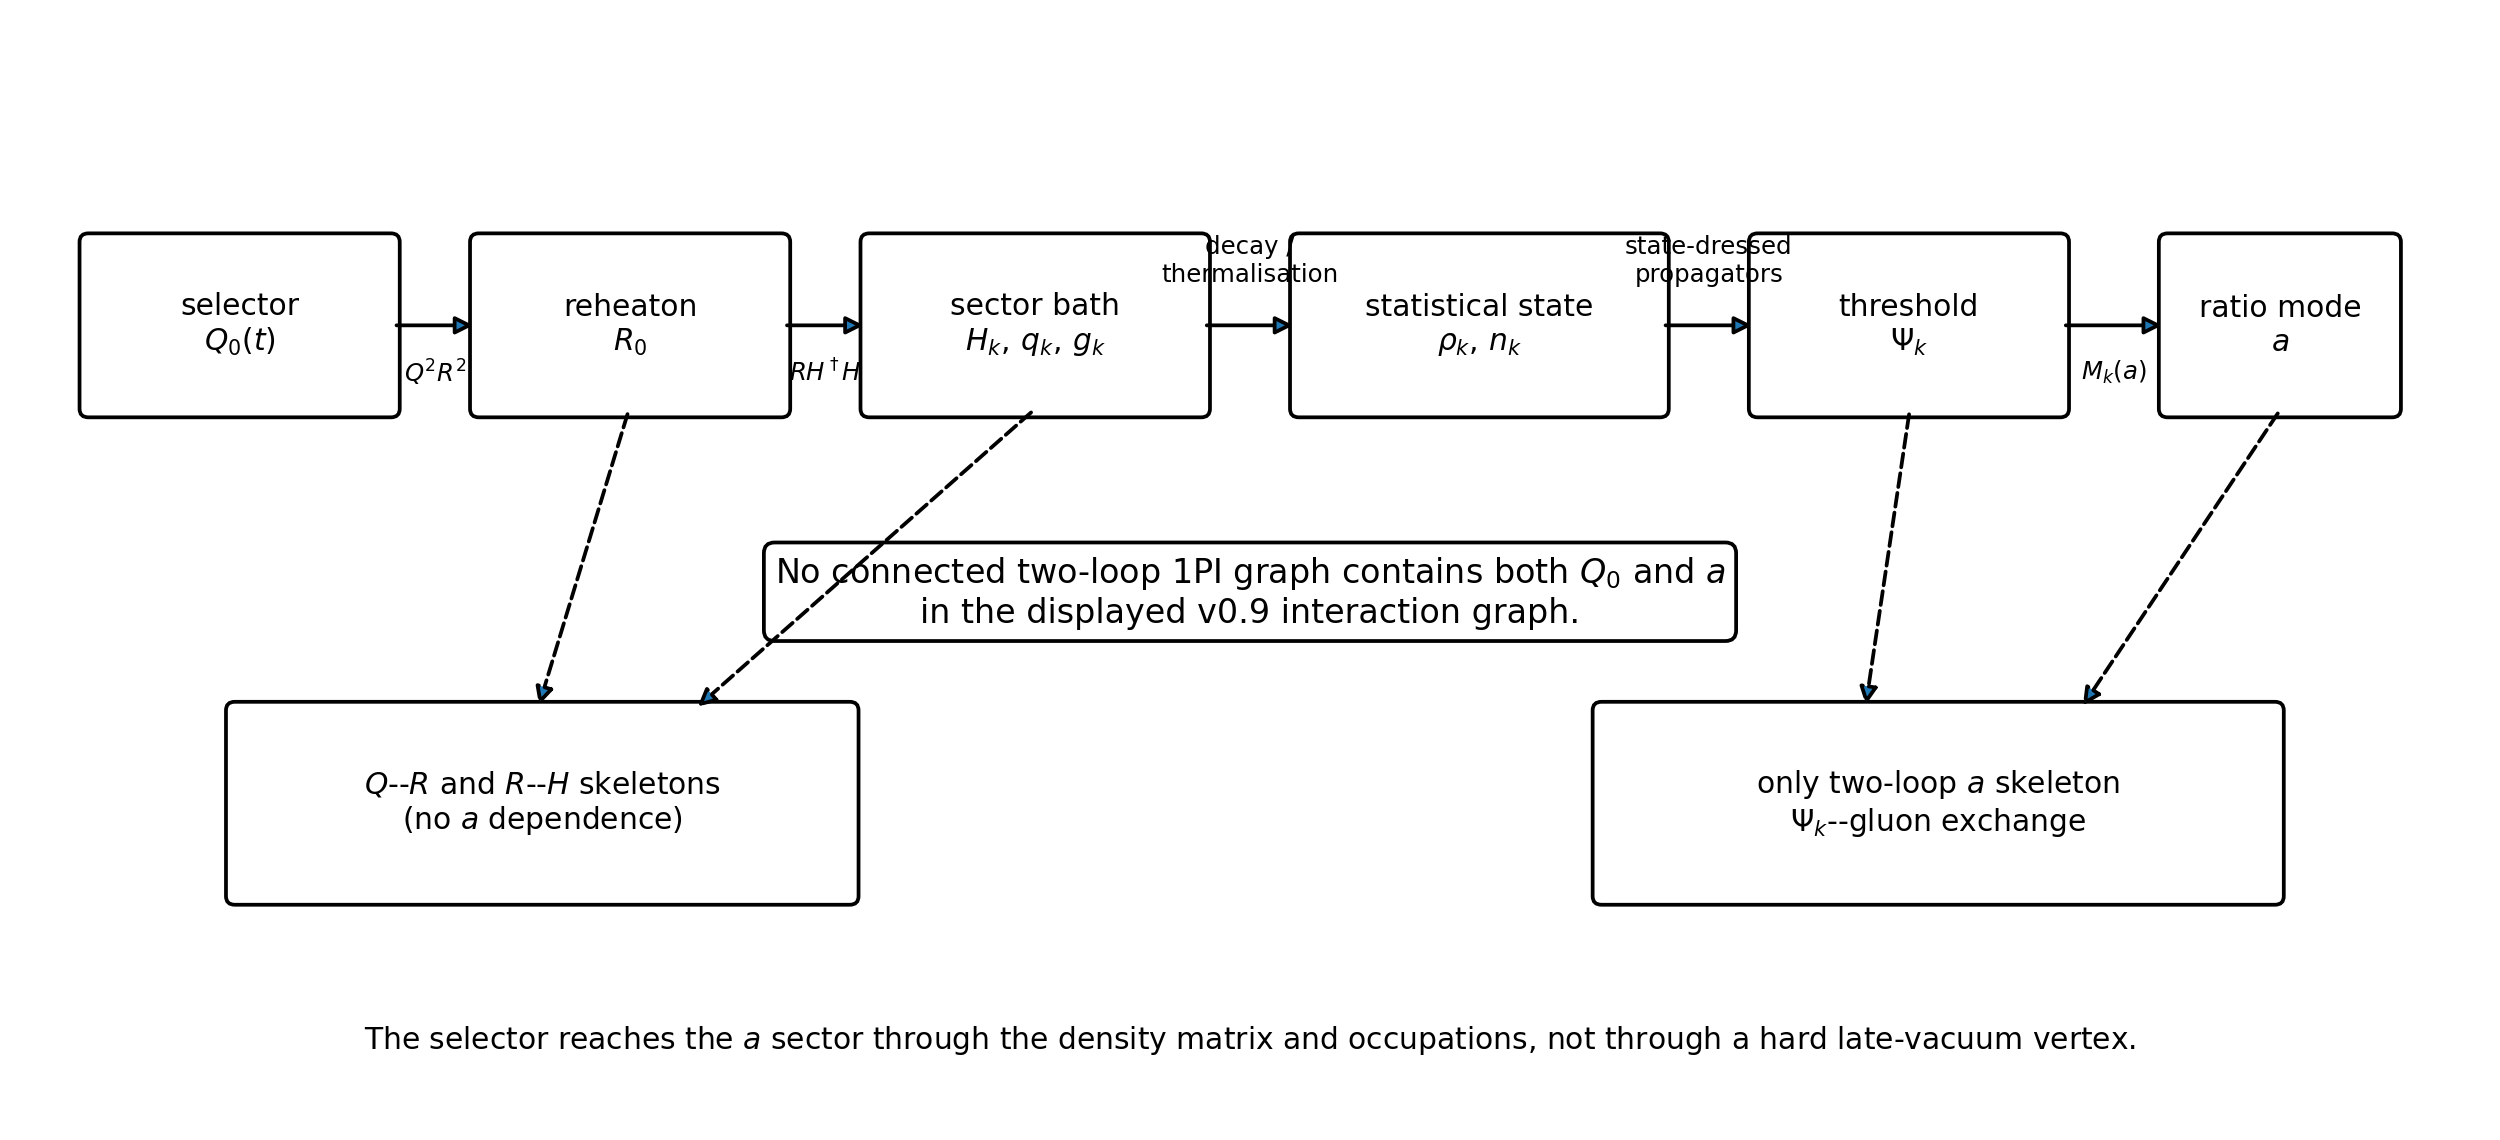
\includegraphics{in_in_two_loop_topology_v1_0.png}
\caption{The displayed interaction graph has no connected two-loop 1PI
skeleton containing both the selector and the ratio mode.}
\end{figure}

\section{3. Closed-time-path
formulation}\label{closed-time-path-formulation}

\subsection{3.1 Generating functional}\label{generating-functional}

Let \texttt{Phi} denote all dynamical fields, including the replicated
sectors, the reheaton orbit, the selector, and the ratio mode. For a
density operator \texttt{rho\_i} specified at the initial matching time
\texttt{t\_i}, the Schwinger--Keldysh generating functional is

\[
Z_{\rho_i}[J_+,J_-;Q_+,Q_-]
=
{\rm Tr}\left[
U_{J_+,Q_+}(t_f,t_i)\,
ho_i\,
U_{J_-,Q_-}^{\dagger}(t_f,t_i)
\right].
\]

Equivalently,

\[
Z_{\rho_i}
=
\int_{\rm CTP}\mathcal D\Phi_+\mathcal D\Phi_-
\;\rho_i[\Phi_+(t_i),\Phi_-(t_i)]
\exp\left
\{iS[\Phi_+,Q_+]-iS[\Phi_-,Q_-]
+iJ_+\Phi_+-iJ_-\Phi_-
\right\}.
\]

The plus and minus fields live on the forward and backward branches of
the closed time contour and are identified at the final turning point.

\subsection{3.2 Replica-covariance
theorem}\label{replica-covariance-theorem}

Let \texttt{Zhat} be the unitary operator that implements the exact
cyclic symmetry. If the action, measure, regulator, and counterterms are
invariant, then

\[
U_{zJ,zQ}=\widehat Z\,U_{J,Q}\,\widehat Z^{-1}.
\]

Cyclicity of the trace gives

\[
Z_{\rho_i}[zJ_+,zJ_-;zQ_+,zQ_-]
=
Z_{\widehat Z^{-1}\rho_i\widehat Z}[J_+,J_-;Q_+,Q_-].
\]

After the Legendre transform, the corresponding effective action obeys

\[
\boxed{
\Gamma_{\widehat Z\rho_i\widehat Z^{-1}}
[z\varphi_+,z\varphi_-;zQ_+,zQ_-]
=
\Gamma_{\rho_i}[\varphi_+,\varphi_-;Q_+,Q_-].
}
\]

This is covariance, not invariance under a field transformation at fixed
asymmetric state.

\subsubsection{Corollary: harmonic coefficients carry state
charge}\label{corollary-harmonic-coefficients-carry-state-charge}

Write a local contribution schematically as

\[
\Gamma_{\rho,Q}^{\rm loc}
\supset
\int d^4x
\sum_{p\in\mathbb Z}
C_p[\rho,Q](x)e^{ipx(x)}.
\]

Replica covariance requires

\[
C_p[z\rho z^{-1},zQ]
=
e^{-2\pi i p/6}C_p[\rho,Q]
\]

up to the sign convention chosen for the cyclic phase shift. Therefore:

\begin{itemize}
\tightlist
\item
  if both \texttt{rho} and \texttt{Q} are cyclic, \texttt{C\_p=0} unless
  \texttt{p} is a multiple of six;
\item
  if the state or background has a nonzero replica Fourier moment, lower
  harmonics are allowed;
\item
  a lower-harmonic coefficient cannot become state independent without a
  persistent symmetry-breaking spurion.
\end{itemize}

Useful state and selector multipoles are

\[
\mathcal N_p(t,\mathbf q)
=
\sum_{k=0}^{5}e^{ip\theta_k}n_k(t,\mathbf q),
\]

and

\[
\mathcal Q_p(t)
=
\sum_{k=0}^{5}e^{ip\theta_k}|Q_k(t)|^2.
\]

The precise sign attached to \texttt{p} depends on the
active-transformation convention. The invariant content is that the
coefficient of \texttt{e\^{}\{ipx\}} must carry the opposite replica
charge.

This theorem is exact and all orders. It does not by itself say that a
state moment decays; it says exactly where any lower harmonic must live.

\section{4. Two-loop topology audit}\label{two-loop-topology-audit}

\subsection{4.1 One-loop structures}\label{one-loop-structures}

At one loop, the \texttt{a} dependence comes from the determinant of the
six heavy fermions,

\[
-i\sum_k{\rm Tr}_{\rm C}\ln
\left(i\gamma^\mu D_{k,\mu}-M_k[a]\right).
\]

In the symmetric vacuum, summing the complete orbit projects this
determinant onto harmonics \texttt{p=6q}.

The selector, reheaton, and Higgs/bath determinants can depend on
\texttt{Q\_0(t)} and on the state, but in the displayed model they have
no direct \texttt{a} dependence.

\subsection{4.2 Two-loop skeletons}\label{two-loop-skeletons}

The two-loop 1PI or 2PI skeletons fall into four classes:

\begin{longtable}[]{@{}
  >{\raggedright\arraybackslash}p{(\columnwidth - 6\tabcolsep) * \real{0.2143}}
  >{\raggedleft\arraybackslash}p{(\columnwidth - 6\tabcolsep) * \real{0.2857}}
  >{\raggedleft\arraybackslash}p{(\columnwidth - 6\tabcolsep) * \real{0.2857}}
  >{\raggedright\arraybackslash}p{(\columnwidth - 6\tabcolsep) * \real{0.2143}}@{}}
\toprule\noalign{}
\begin{minipage}[b]{\linewidth}\raggedright
Skeleton class
\end{minipage} & \begin{minipage}[b]{\linewidth}\raggedleft
Contains \texttt{Q}?
\end{minipage} & \begin{minipage}[b]{\linewidth}\raggedleft
Contains \texttt{a}?
\end{minipage} & \begin{minipage}[b]{\linewidth}\raggedright
Effect
\end{minipage} \\
\midrule\noalign{}
\endhead
\bottomrule\noalign{}
\endlastfoot
selector--reheaton double bubble or sunset & yes & no & transient
selector/reheaton masses and damping \\
reheaton--Higgs/bath skeleton & indirectly & no & prepares
sector-dependent occupations \\
pure gluon/ghost skeleton & no & no & contributes to pressure but not
directly to \texttt{delta\ Gamma/delta\ a} \\
heavy-fermion--gluon exchange & through state only & yes & NLO QCD
correction to the \texttt{a} force \\
\end{longtable}

A connected two-loop graph containing \texttt{Q\_0} and \texttt{a} would
need a renormalizable vertex shared by the selector/reheaton graph and
the heavy threshold. The displayed v0.9 action has no such vertex.
Connecting the two sides through the sector bath requires additional
interaction vertices and at least one higher loop.

Therefore:

\[
\boxed{
\Gamma_{Q-a}^{\rm 1PI,(2\ loop)}=0
\quad\text{for the displayed interaction graph.}
}
\]

This is a topology statement, not a claim that all higher-loop portal
graphs vanish. The first nonzero mixed order depends on the decay
operators assigned to \texttt{Psi\_k} and on the UV completion of the
Higgs thermalizer.

\section{5. Two-loop 2PI/CTP effective
action}\label{two-loop-2pictp-effective-action}

\subsection{5.1 QCD sector}\label{qcd-sector}

Let \texttt{S\_k\^{}\{ab\}} and \texttt{D\_\{k,mu\ nu\}\^{}\{ab\}}
denote the contour-ordered heavy-fermion and gluon propagators, where
the contour indices take values \texttt{+} and \texttt{-}. The two-loop
fermion--gluon contribution can be written compactly as

\[
\boxed{
\Gamma_{2,{\rm QCD}}^{(2)}
=
-\frac{i g_s^2}{2}
\sum_{k=0}^{5}
\int_{\rm C}d^4x\,d^4y\;
{\rm tr}\left[
\gamma^\mu T^A S_k(x,y)
\gamma^\nu T^B S_k(y,x)
\right]
D^{AB}_{k,\mu\nu}(x,y).
}
\]

Gauge-fixing, ghost, and pure-glue skeletons complete the two-loop QCD
functional but carry no explicit \texttt{a} dependence. At the
stationary propagators,

\[
\frac{\delta\Gamma}{\delta S_k}=0,
\qquad
\frac{\delta\Gamma}{\delta D_k}=0.
\]

The implicit \texttt{a} derivatives of the dressed propagators therefore
drop out of the field equation. Taking the physical limit
\texttt{a\_+=a\_-=a} yields

\[
\boxed{
\Box a+V_0'(a)
+
\sum_{k=0}^{5}
M_k'(a)
\langle\bar\Psi_k\Psi_k\rangle_{\rho,{\rm ren}}
=0,
}
\]

where the condensate includes the one-loop statistical contribution and
its two-loop QCD correction.

This equation is the real-time generalization of differentiating the
equilibrium free energy with respect to the mass.

\subsection{5.2 Influence-functional
expansion}\label{influence-functional-expansion}

Define the mass source

\[
j_k[a](x)
\equiv
M_k[a(x)]-M,
\]

and the composite operator

\[
O_k(x)=\bar\Psi_k\Psi_k.
\]

In the Keldysh average/difference basis,

\[
j_{k,r}=\frac12(j_{k,+}+j_{k,-}),
\qquad
j_{k,a}=j_{k,+}-j_{k,-},
\]

the influence action through quadratic order in the source is

\[
\begin{aligned}
\Gamma_{\rm IF}={}&
-\sum_k\int d^4x\;
 j_{k,a}(x)\langle O_k(x)\rangle_\rho
\\
&-\sum_k\int d^4x\,d^4y\;
 j_{k,a}(x)G^R_{OO,k}(x,y)j_{k,r}(y)
\\
&+\frac{i}{2}\sum_k\int d^4x\,d^4y\;
 j_{k,a}(x)G^H_{OO,k}(x,y)j_{k,a}(y)
+O(j^3).
\end{aligned}
\]

The three terms have distinct meanings:

\begin{itemize}
\tightlist
\item
  \texttt{⟨O\_k⟩} gives the local state-dependent drift or potential;
\item
  \texttt{G\^{}R} gives nonlocal response, dissipation, and memory;
\item
  \texttt{G\^{}H} gives noise and decoherence.
\end{itemize}

A vacuum Wilson coefficient, a finite-density potential, and a memory
kernel are therefore not interchangeable descriptions of the same
object.

\section{6. Vacuum/state decomposition}\label{vacuumstate-decomposition}

Write each full propagator as

\[
S_k=S_{k,{\rm vac}}+\delta S_{k,\rho},
\qquad
D_k=D_{k,{\rm vac}}+\delta D_{k,\rho}.
\]

The two-loop exchange functional then separates into:

\begin{enumerate}
\def\labelenumi{\arabic{enumi}.}
\tightlist
\item
  an all-vacuum term \texttt{S\_vac\ S\_vac\ D\_vac};
\item
  terms with one statistical insertion;
\item
  terms with two or three statistical insertions.
\end{enumerate}

\subsection{6.1 Vacuum term}\label{vacuum-term}

The all-vacuum term is the same functional of \texttt{M\_k(a)} in every
replicated sector:

\[
\Gamma_{\rm vac}^{(2)}[a]
=
\sum_{k=0}^{5}
\mathcal F_{\rm vac}^{(2)}(M_k(a),g_s,\mu).
\]

Under \texttt{x\ -\textgreater{}\ x+2\ pi/6}, the set of masses is
permuted. Hence

\[
\Gamma_{\rm vac}^{(2)}
\left(x+\frac{2\pi}{6}\right)
=
\Gamma_{\rm vac}^{(2)}(x).
\]

Its Fourier series contains only

\[
p=0,\pm6,\pm12,\ldots.
\]

Because every insertion of \texttt{e\^{}\{+ix\}} or
\texttt{e\^{}\{-ix\}} comes with one factor of \texttt{epsilon}, the
first nonconstant term remains \texttt{O(epsilon\^{}6)}.

A symbolic root-of-unity expansion through \texttt{epsilon\^{}10} and a
numerical Fourier transform of a representative one-plus-two-loop
analytic sector functional both confirm this selection rule. The largest
numerical amplitude among \texttt{p=1,...,5} is \texttt{5.09e-8} of the
\texttt{p=6} amplitude, consistent with floating-point cancellation of
an exactly vanishing result.

\begin{figure}
\centering
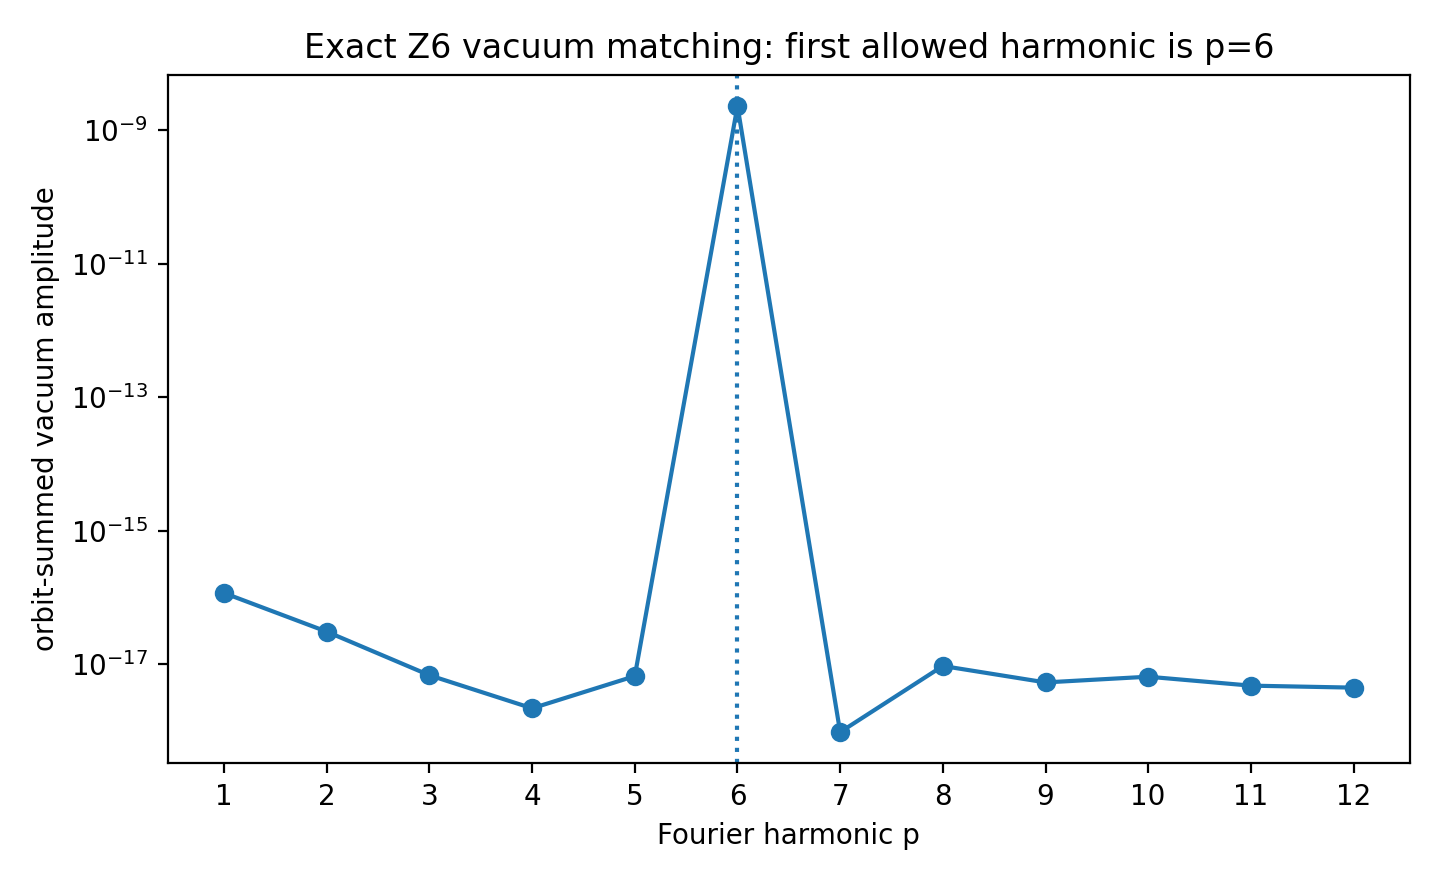
\includegraphics{in_in_vacuum_harmonics_v1_0.png}
\caption{The complete vacuum orbit eliminates the forbidden harmonics;
the first allowed nonconstant mode is p = 6.}
\end{figure}

\subsection{6.2 State terms}\label{state-terms}

A statistical insertion contains an occupation function or a
non-equilibrium correlator specific to sector \texttt{k}. The sector sum
is then weighted:

\[
\Gamma_{\rm state}
\sim
\sum_k
\mathcal W_k[\rho]
\mathcal F(M_k(a)).
\]

If the weights are unequal, the root-of-unity projector no longer
annihilates the lower harmonics. This is not a radiative failure; it is
the intended finite-density effect.

At first order in \texttt{epsilon},

\[
\Gamma_{\rm state}^{(p=1)}
\propto
{\rm Re}\left[
e^{ix}
\sum_k\mathcal W_k e^{i\theta_k}
\right].
\]

The coefficient is exactly the first replica Fourier moment of the
state. It vanishes when the state becomes cyclic, and it redshifts or
Boltzmann suppresses when the corresponding particles disappear.

\subsection{6.3 Ultraviolet structure}\label{ultraviolet-structure}

For a UV-soft or Hadamard state, the statistical additions
\texttt{delta\ S\_rho} and \texttt{delta\ D\_rho} vanish sufficiently
rapidly at large momentum. Diagrams containing at least one such
insertion are then UV finite after the usual vacuum subdivergences are
removed. The divergent bulk part is the vacuum part and therefore
preserves the exact cyclic symmetry.

If one imposes a general effective state at a finite matching surface,
additional divergences may occur. They are localized on that initial
surface and are removed by boundary counterterms. They renormalize the
state specification, not a late-time sector-asymmetric bulk coupling.

\section{7. Explicit NLO thermal
harmonic}\label{explicit-nlo-thermal-harmonic}

\subsection{7.1 High-temperature
pressure}\label{high-temperature-pressure}

In a locally thermal and slowly varying regime, the static limit of the
CTP effective action is the thermal free energy. For one massive Dirac
colour triplet at zero chemical potential, the mass-dependent
high-temperature pressure through NLO can be written

\[
P_k(T_k,M_k)
=
P_{k,0}
-
N_cM_k^2T_k^2
\left[
\frac1{12}
+
(4\pi\alpha_{s,k})C_F C_T(\bar\mu/T_k)
\right]
+
O(M_k^4),
\]

where

\[
C_T(r)
=
J_3(0)
+
\frac{1}{48\pi^2}
\left[
\frac12+3\ln\left(
\frac{r e^{\gamma_E}}{\pi}
\right)
\right],
\]

and

\[
J_3(0)=-0.00129532.
\]

Defining

\[
r_k
=
12(4\pi\alpha_{s,k})C_F C_T(\bar\mu/T_k),
\]

the first harmonic of the effective potential \texttt{V=-P} is

\[
\boxed{
V_{\rm state}^{(1+2)}(x)
=
-\frac{N_cM^2\epsilon}{6}
{\rm Re}\left[
e^{ix}
\sum_{k=0}^{5}T_k^2(1+r_k)e^{i\theta_k}
\right]
+O(\epsilon^2).
}
\]

This is the two-loop correction to the same state phasor used in v0.8
and v0.9.

\subsection{7.2 Benchmark}\label{benchmark}

Use

\[
M=1.002\times10^6\ {\rm GeV},
\qquad
T_0=1.002\times10^8\ {\rm GeV},
\qquad
T_5=T_0/4,
\]

with the remaining sectors empty and \texttt{epsilon\ =\ 2.70e-13}. At
\texttt{bar\ mu\ =\ 2\ pi\ T}, one-loop running gives

\[
\alpha_{s,0}=0.0393544,
\qquad
\alpha_{s,5}=0.0416445,
\]

and hence

\[
r_0=0.0617566,
\qquad
r_5=0.0653504.
\]

The leading phasor is

\[
\frac{W_{\rm LO}}{T_0^2}
=
1+\frac1{16}e^{i5\pi/3},
\]

with

\[
|W_{\rm LO}|=1.03266948,
\qquad
\arg W_{\rm LO}=-0.05243827.
\]

At NLO,

\[
|W_{\rm NLO}|=1.09656599,
\qquad
\arg W_{\rm NLO}=-0.05261005.
\]

Therefore,

\[
\boxed{
\frac{|W_{\rm NLO}|}{|W_{\rm LO}|}=1.061875,
}
\]

and

\[
\boxed{
\Delta\arg W=-1.7178\times10^{-4}\ {\rm rad}
=-0.009842^\circ.
}
\]

The NLO correction strengthens the focusing amplitude by approximately
\texttt{6.19\%} and barely rotates the selected phase.

The corresponding first-harmonic free-energy amplitudes are

\[
|V_{p=1}^{\rm LO}|=1.4053\times10^{15}\ {\rm GeV}^4,
\]

and

\[
|V_{p=1}^{\rm NLO}|=1.4922\times10^{15}\ {\rm GeV}^4.
\]

For comparison, the protected zero-temperature \texttt{p=6} coefficient
at the same benchmark is

\[
|V_{p=6}^{\rm vac}|=9.27\times10^{-56}\ {\rm GeV}^4.
\]

The enormous ratio is expected: the early thermal state is intentionally
allowed to choose a branch, while the vacuum potential is protected to
sixth spurion order.

\subsection{7.3 Renormalization-scale
band}\label{renormalization-scale-band}

\begin{longtable}[]{@{}lrr@{}}
\toprule\noalign{}
Scale & Amplitude ratio \texttt{NLO/LO} & Selected phasor phase \\
\midrule\noalign{}
\endhead
\bottomrule\noalign{}
\endlastfoot
\texttt{bar\ mu\ =\ pi\ T} & 1.02784 & -0.0525205 rad \\
\texttt{bar\ mu\ =\ 2\ pi\ T} & 1.06188 & -0.0526100 rad \\
\texttt{bar\ mu\ =\ 4\ pi\ T} & 1.09408 & -0.0526846 rad \\
\end{longtable}

The phase is more stable than the amplitude. A complete HTL-resummed and
time-dependent calculation would reduce the residual scale ambiguity,
but nothing in this band suggests a qualitative loss of focusing.

\section{8. Decay of the state
harmonic}\label{decay-of-the-state-harmonic}

The exact one-loop scalar-density integral was used to follow the
heavy-threshold force as the populated-sector temperatures redshift. At
early times the force scales approximately as
\texttt{M\^{}2\ T\^{}2\ epsilon}. When \texttt{T\_0} reaches \texttt{M},
at scale factor

\[
\frac{a}{a_R}=\frac{T_0}{M}=100,
\]

Boltzmann suppression begins to dominate. By \texttt{a/a\_R\ =\ 3e4},
the normalized first-harmonic amplitude is

\[
1.44\times10^{-138}
\]

at one loop and

\[
1.36\times10^{-138}
\]

with the NLO correction used in its domain of validity.

\begin{figure}
\centering
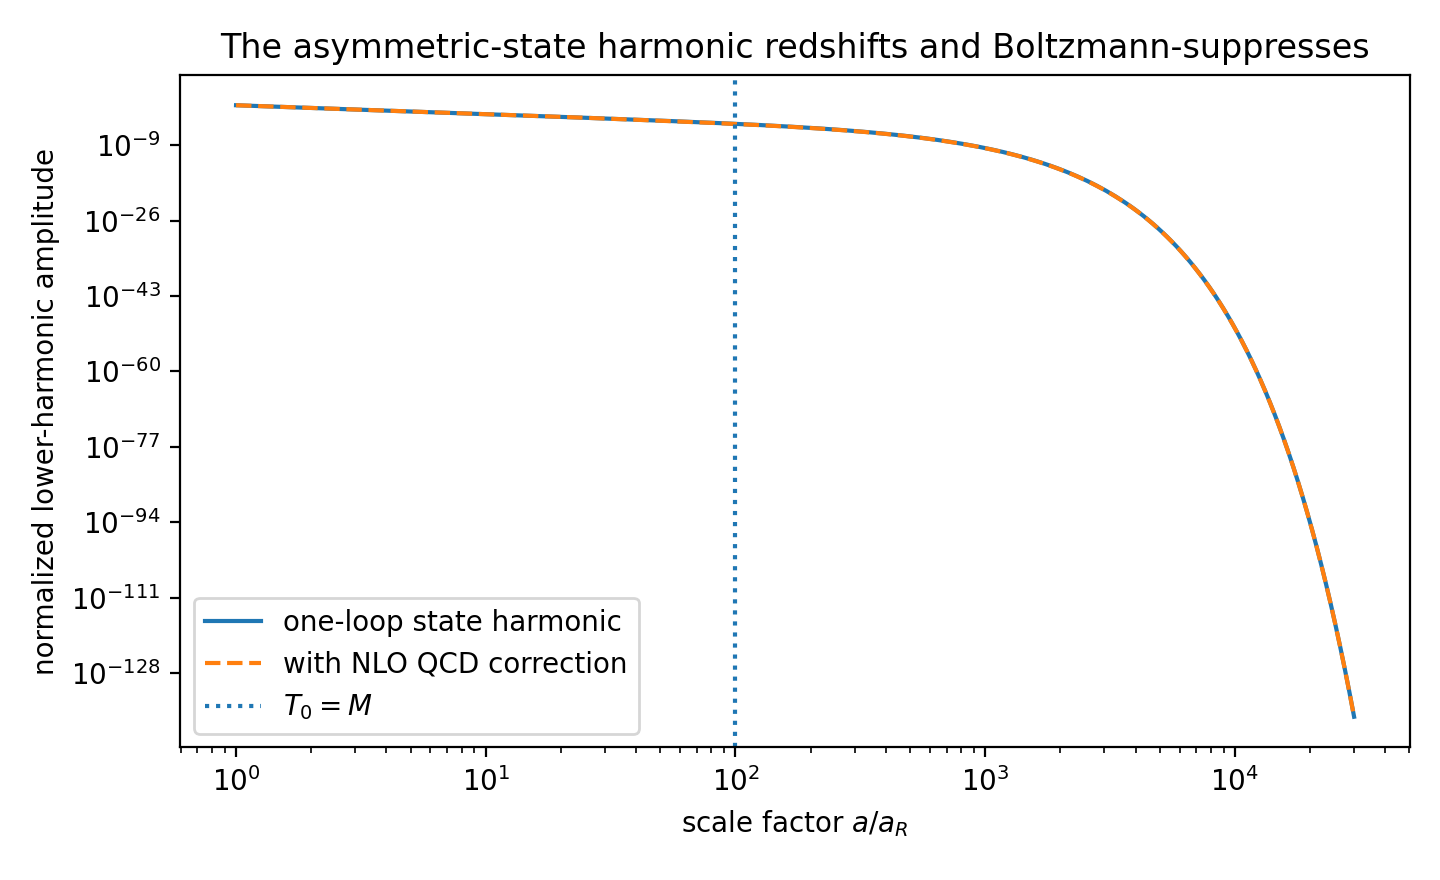
\includegraphics{in_in_state_harmonic_decay_v1_0.png}
\caption{The heavy-threshold state harmonic redshifts and becomes
exponentially suppressed; the NLO correction changes the finite
coefficient but not the fate of the term.}
\end{figure}

This conclusion is specific to the heavy-threshold contribution. Later
QCD trace-anomaly and baryonic finite-density terms can persist much
longer and are part of the cosmological vacuum-selection mechanism. They
remain state-dependent source terms proportional to physical densities;
they are not vacuum matching coefficients.

\section{9. Selector disappearance and state
persistence}\label{selector-disappearance-and-state-persistence}

The selector and the state occupy different temporal roles. With the
benchmark widths, the selector order parameter falls rapidly, while the
selected reheaton population remains. The daughter-state asymmetry is
therefore produced primarily after the hard background has disappeared.

\begin{figure}
\centering
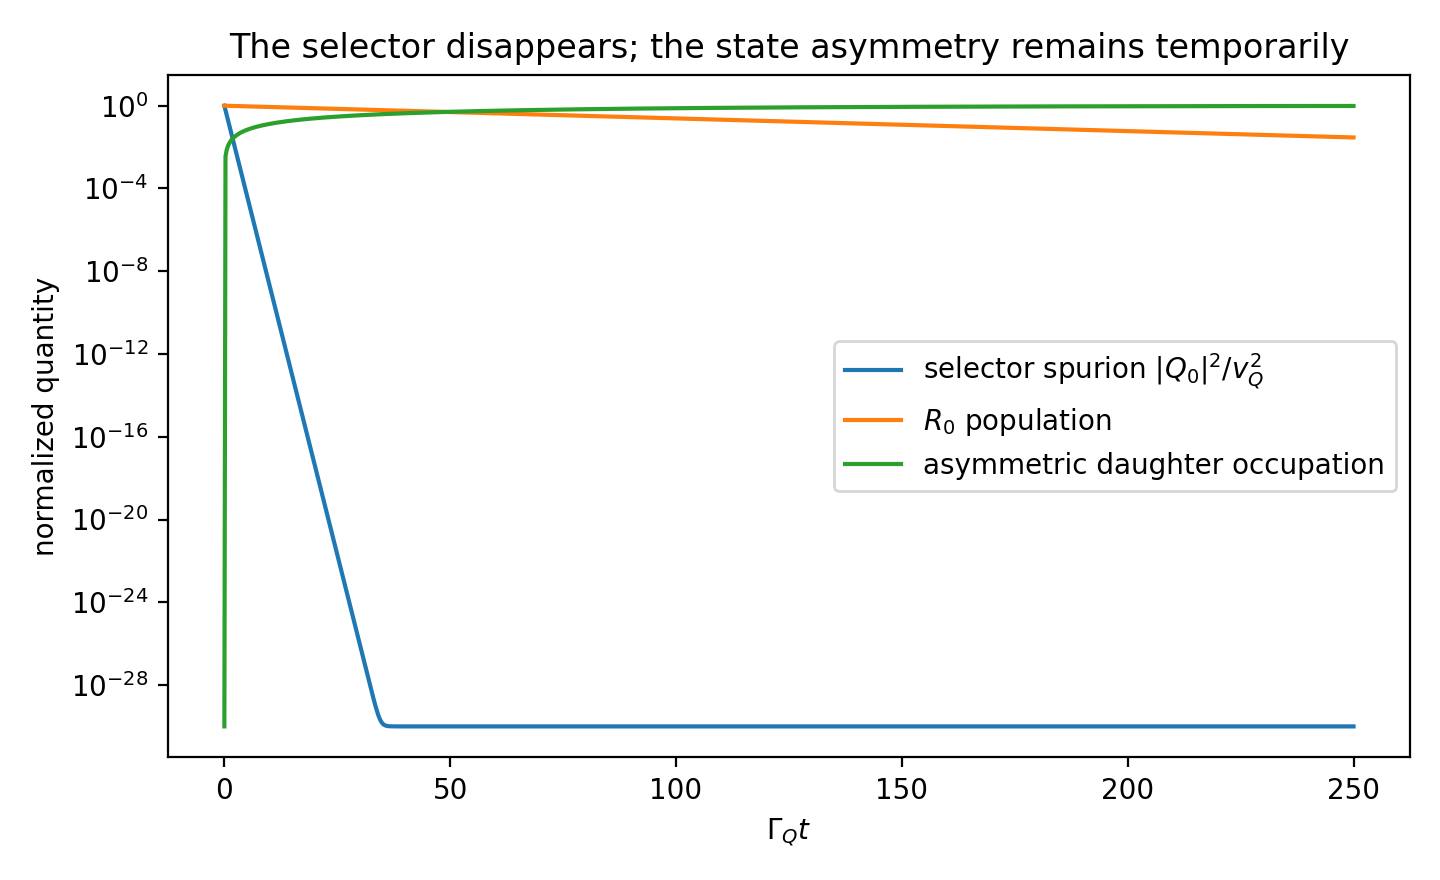
\includegraphics{in_in_selector_state_separation_v1_0.png}
\caption{The selector background disappears before most reheaton decays,
while the selected reheaton and its daughter occupation retain the
replica label.}
\end{figure}

The figure uses a simple exponential timing model. It establishes the
hierarchy but does not replace a non-equilibrium solution for the
rolling selector and reheaton occupation numbers.

\section{10. Nonlocal memory, dissipation, and
noise}\label{nonlocal-memory-dissipation-and-noise}

\subsection{10.1 Spectral representation}\label{spectral-representation}

For a stationary or slowly varying bath, the retarded kernel admits a
spectral representation of the form

\[
K_R(t-t')
=
\theta(t-t')
\int_0^\infty\frac{d\omega}{\pi}
\rho_K(\omega)
\sin\left[\omega(t-t')\right].
\]

If the spectral density has no zero-frequency delta function or
nonintegrable singularity, phase mixing implies that the kernel decays
at late separation. A numerical representative with a two-particle
threshold gives

\[
\frac{{\rm RMS}_{\rm late}}{{\rm RMS}_{\rm early}}
=1.76\times10^{-6}.
\]

\begin{figure}
\centering
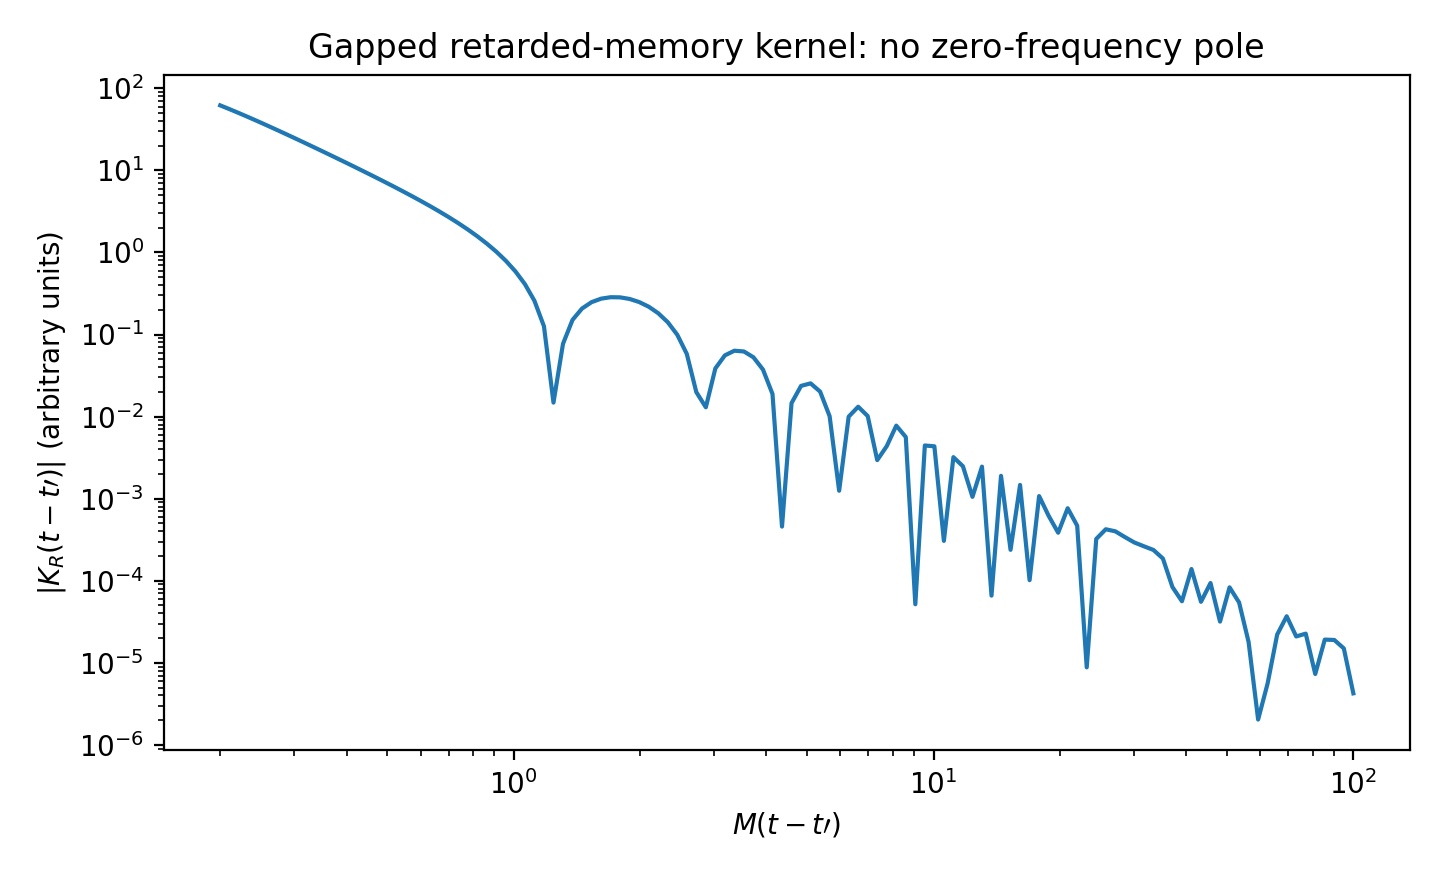
\includegraphics{in_in_memory_kernel_v1_0.png}
\caption{A representative gapped retarded kernel dephases at late time
when no zero-frequency pole is present.}
\end{figure}

The calculation is intentionally diagnostic, not a claim that the hot
QCD kernel is literally gapped. In a thermal plasma, scattering cuts and
hydrodynamic poles can produce power-law or long-lived tails. Such
contributions are tied to conserved densities and occupations. They may
preserve a finite-density force, but they still do not become a
state-independent vacuum coefficient.

\subsection{10.2 What can survive}\label{what-can-survive}

A late effect can survive if one of the following remains:

\begin{itemize}
\tightlist
\item
  a conserved sector number carried by a stable relic;
\item
  a stable asymmetric condensate;
\item
  a topological or hydrodynamic zero mode;
\item
  a permanent selector expectation value;
\item
  a hard symmetry-breaking coupling;
\item
  an anomaly that violates the cyclic symmetry.
\end{itemize}

The first three are state variables or order parameters. The last three
would be genuine failures of the proposed escape hatch.

A transient force may also displace \texttt{a} and leave coherent
oscillations after the force turns off. That is a changed initial
condition for the symmetric late-time theory, not a new lower-harmonic
vacuum operator.

\section{11. Initial-state and matching-surface
renormalization}\label{initial-state-and-matching-surface-renormalization}

A practical calculation often integrates out the selector/reheaton era
and starts the lower-energy evolution at a finite time \texttt{t\_star}
with a reduced density matrix. The short-distance structure of that
matrix matters.

For a physical UV-soft state, the high-momentum correlators approach the
interacting vacuum correlators, so the ordinary bulk counterterms
suffice. For a more general effective state, loop diagrams can produce
divergences localized at \texttt{t\_star}. They are removed by local
boundary operators in the density-matrix action, for example Gaussian
terms schematically of the form

\[
S_{\rm bdry}
=
\frac12\int_{t=t_\star}d^3x\,d^3y
\left[
\Phi_+ A\Phi_+
-\Phi_- A^*\Phi_-
+2i\Phi_+B\Phi_-
\right].
\]

Replica covariance requires these boundary kernels to transform with the
state. A one-hot or sector-asymmetric boundary counterterm is therefore
allowed if it renormalizes the asymmetric state. Its support remains on
the matching surface.

The key distinction is:

\[
\boxed{
\text{boundary renormalization of }\rho
\ne
\text{bulk renormalization of the late vacuum Hamiltonian}.
}
\]

\section{12. Operator audit and the phase-sequestering
condition}\label{operator-audit-and-the-phase-sequestering-condition}

\subsection{12.1 Exact cyclic symmetry is necessary but
insufficient}\label{exact-cyclic-symmetry-is-necessary-but-insufficient}

Construct selector Fourier composites

\[
\mathcal Q_p
=
\sum_{k=0}^{5}e^{ip\theta_k}|Q_k|^2.
\]

Because \texttt{mathcal\ Q\_p} carries replica charge, the local
operator

\[
\boxed{
\Delta\mathcal L_{p,Q}
=
c_{p,Q}\epsilon^p
 e^{ipx}\mathcal Q_{-p}
+\text{h.c.}
}
\]

is cyclically invariant for \texttt{p=1,...,5}. On the one-hot branch it
generates a transient lower harmonic. When every \texttt{Q\_k} returns
to zero, it vanishes.

The problem would be more serious if the same operator could be
generated without the factor \texttt{epsilon\^{}p}, or if integrating
out the selector left behind a \texttt{Q}-independent coefficient. To
prevent that, the theory must satisfy:

\[
\boxed{
\epsilon\to0
\quad\Longrightarrow\quad
U(1)_a\text{ shift symmetry is restored.}
}
\]

Every local nonderivative dependence on \texttt{a} must then contain the
appropriate number of explicit shift-breaking spurions. This is the
\textbf{phase-sequestering condition}.

\subsection{12.2 Recommended UV
implementation}\label{recommended-uv-implementation}

The strongest implementation is to make \texttt{a} a Wilson-line or
collective pNGB for which:

\begin{itemize}
\tightlist
\item
  local selector/reheaton operators cannot depend directly on the
  complete phase;
\item
  the mass orbit is generated only by a complete messenger chain;
\item
  breaking the phase symmetry requires the same replicated spurions that
  produce \texttt{M\_k(a)};
\item
  the residual \texttt{Z\_6} is an anomaly-free discrete gauge symmetry
  rather than a merely global one.
\end{itemize}

This converts the empirical absence of a portal into a structural
selection rule.

\subsection{12.3 Dangerous operator
classes}\label{dangerous-operator-classes}

\begin{longtable}[]{@{}
  >{\raggedright\arraybackslash}p{(\columnwidth - 6\tabcolsep) * \real{0.2143}}
  >{\raggedleft\arraybackslash}p{(\columnwidth - 6\tabcolsep) * \real{0.2857}}
  >{\raggedleft\arraybackslash}p{(\columnwidth - 6\tabcolsep) * \real{0.2857}}
  >{\raggedright\arraybackslash}p{(\columnwidth - 6\tabcolsep) * \real{0.2143}}@{}}
\toprule\noalign{}
\begin{minipage}[b]{\linewidth}\raggedright
Operator or effect
\end{minipage} & \begin{minipage}[b]{\linewidth}\raggedleft
Allowed by exact \texttt{Z6}?
\end{minipage} & \begin{minipage}[b]{\linewidth}\raggedleft
Persists at \texttt{Q=0}?
\end{minipage} & \begin{minipage}[b]{\linewidth}\raggedright
Verdict
\end{minipage} \\
\midrule\noalign{}
\endhead
\bottomrule\noalign{}
\endlastfoot
\texttt{epsilon\^{}p\ e\^{}\{ipx\}\ mathcal\ Q\_\{-p\}} & yes & no &
acceptable transient focusing \\
\texttt{epsilon\^{}p\ e\^{}\{ipx\}\ mathcal\ N\_\{-p\}} & yes & while
state persists & acceptable finite-density force \\
\texttt{epsilon\^{}p\ e\^{}\{ipx\}} for \texttt{p=1,...,5} & no & yes &
forbidden if symmetry exact \\
sector-dependent mass/coupling left after \texttt{Q-\textgreater{}0} &
no & yes & hard failure \\
stable charged condensate & state-dependent & yes & model-dependent
persistent source \\
initial-surface counterterm & yes for asymmetric state & boundary only &
acceptable if renormalized \\
anomaly-induced cyclic breaking & possible in bad UV completion & yes &
hard failure \\
\end{longtable}

\section{13. What the two-loop calculation has and has not
proved}\label{what-the-two-loop-calculation-has-and-has-not-proved}

\subsection{13.1 Proved or explicitly
checked}\label{proved-or-explicitly-checked}

\begin{enumerate}
\def\labelenumi{\arabic{enumi}.}
\tightlist
\item
  \textbf{CTP covariance:} the exact effective action transforms
  covariantly with the density matrix; a fixed asymmetric state may
  possess lower harmonics without violating the microscopic symmetry.
\item
  \textbf{Topology:} no connected two-loop 1PI graph contains both
  \texttt{Q\_0} and \texttt{a} in the displayed v0.9 interaction graph.
\item
  \textbf{Vacuum protection:} the one- and two-loop vacuum sector sum
  contains no \texttt{p=1,...,5} harmonic.
\item
  \textbf{State localization:} every lower harmonic at two loops
  contains a state or transient-background insertion.
\item
  \textbf{Thermal NLO stability:} QCD increases the focusing amplitude
  by about \texttt{6\%} and shifts the phase by only
  \texttt{0.01\ degrees} at the central scale.
\item
  \textbf{Late matching:} the heavy-threshold state harmonic is removed
  by redshift and Boltzmann suppression.
\item
  \textbf{Memory condition:} without a zero-frequency pole, a transient
  retarded memory kernel dephases.
\item
  \textbf{Renormalization structure:} UV divergences from a general
  initial state are boundary localized; bulk vacuum counterterms retain
  the cyclic symmetry.
\end{enumerate}

\subsection{13.2 Not yet proved}\label{not-yet-proved}

\begin{enumerate}
\def\labelenumi{\arabic{enumi}.}
\tightlist
\item
  An all-orders theorem excluding every mixed selector--threshold bulk
  operator in a specified UV completion.
\item
  The exact first nonzero loop order of direct \texttt{Q}--\texttt{a}
  communication once all vectorlike-fermion decay operators are
  supplied.
\item
  A full two-loop Kadanoff--Baym solution for the nonthermal selector,
  reheaton, Higgs, quark, gluon, and threshold distributions.
\item
  Nonperturbative preheating and resonance production of nominally
  inaccessible replica sectors.
\item
  Absence of anomalies in the proposed discrete-gauge embedding.
\item
  The fate of long-time hydrodynamic tails in the actual expanding
  plasma.
\end{enumerate}

\section{14. Acceptance matrix}\label{acceptance-matrix}

\begin{longtable}[]{@{}
  >{\raggedright\arraybackslash}p{(\columnwidth - 4\tabcolsep) * \real{0.3000}}
  >{\raggedleft\arraybackslash}p{(\columnwidth - 4\tabcolsep) * \real{0.4000}}
  >{\raggedright\arraybackslash}p{(\columnwidth - 4\tabcolsep) * \real{0.3000}}@{}}
\toprule\noalign{}
\begin{minipage}[b]{\linewidth}\raggedright
Requirement
\end{minipage} & \begin{minipage}[b]{\linewidth}\raggedleft
Verdict
\end{minipage} & \begin{minipage}[b]{\linewidth}\raggedright
Reason
\end{minipage} \\
\midrule\noalign{}
\endhead
\bottomrule\noalign{}
\endlastfoot
exact cyclic bulk counterterms & \textbf{PASS} & vacuum divergences are
sector-orbit sums \\
forbidden vacuum harmonics through two loops & \textbf{PASS} &
root-of-unity selection and numerical Fourier check \\
no direct two-loop selector--ratio skeleton & \textbf{PASS} & absent
from displayed interaction graph \\
intended finite-density first harmonic & \textbf{PASS} & generated by
replica Fourier moment of the state \\
NLO QCD control at benchmark & \textbf{PASS} & \texttt{6.19\%}
correction at central scale \\
phase stability & \textbf{PASS} & \texttt{0.00984\ degrees} shift \\
selector removed before most reheaton decay & \textbf{PASS} & only
\texttt{1.40\%} decays in one selector lifetime \\
heavy-threshold state term disappears & \textbf{PASS} & redshift plus
Boltzmann suppression \\
gapped memory disappears & \textbf{PASS conditional} & no zero-frequency
pole \\
initial-state renormalization & \textbf{PASS conditional} & requires
UV-soft state or boundary counterterms \\
exact \texttt{Z6} alone protects every transient operator &
\textbf{FAIL} & charged selector composites permit transient low
harmonics \\
phase sequestering & \textbf{REQUIRED} & must be enforced by UV
symmetry/geometry \\
all-orders radiative escape & \textbf{OPEN} & requires higher-loop
portal theorem \\
nonperturbative reheating & \textbf{OPEN} & requires lattice or
Kadanoff--Baym simulation \\
\end{longtable}

\section{15. Novelty boundary}\label{novelty-boundary}

The ingredients are individually established:

\begin{itemize}
\tightlist
\item
  the Schwinger--Keldysh treatment of mixed and nonequilibrium states;
\item
  boundary renormalization of effective initial states;
\item
  symmetry-preserving 2PI truncations for linearly realized global
  symmetries;
\item
  cyclic suppression of vacuum harmonics with an unsuppressed
  finite-density force;
\item
  the NLO massive-quark pressure;
\item
  state-induced symmetry breaking with a symmetric Hamiltonian.
\end{itemize}

The candidate contribution is the combined result:

\[
\boxed{
\begin{gathered}
\text{exact cyclic threshold protection}
+
\text{transient state-selected reheating}
\\
+
\text{CTP replica-covariance theorem}
+
\text{two-loop topology separation}
\\
+
\text{NLO QCD phasor stability}
+
\text{chronometric-shear interpretation}.
\end{gathered}
}
\]

The targeted literature search found direct precedent for
state-generated finite-density potentials and direct warnings that a
hard asymmetric reheating spurion radiatively produces lower vacuum
harmonics. It did not reveal the exact
selector/reheaton/visible-QCD/chronometric package above. That is a
candidate priority claim, not yet a definitive one.

\section{16. Next decisive calculation}\label{next-decisive-calculation}

The positive two-loop result moves the bottleneck upward rather than
eliminating it. The next calculation should have two linked parts.

\subsection{16.1 First mixed selector--threshold matching
order}\label{first-mixed-selectorthreshold-matching-order}

Specify the complete vectorlike-fermion decay operators and the UV
thermalizer. Enumerate all connected 1PI graphs containing:

\begin{itemize}
\tightlist
\item
  at least one selector insertion;
\item
  at least one shift-breaking heavy-threshold insertion;
\item
  enough sector-bath connectors to join them.
\end{itemize}

Then calculate the first nonzero coefficient of

\[
\epsilon^p e^{ipx}\mathcal Q_{-p}
\]

and prove that it vanishes with \texttt{Q} and cannot match onto a
\texttt{Q}-independent \texttt{p\textless{}6} operator. This is likely a
three-loop-or-higher problem, but the precise order is portal dependent.

\subsection{16.2 Nonthermal Kadanoff--Baym
evolution}\label{nonthermal-kadanoffbaym-evolution}

Evolve the coupled statistical and spectral functions for

\[
Q_k,
\quad R_k,
\quad H_k,
\quad\Psi_k,
\quad g_k
\]

through selector restoration and reheaton decay. The simulation must
determine:

\begin{itemize}
\tightlist
\item
  whether sectors \texttt{1,2,3,4} remain unpopulated beyond
  perturbative estimates;
\item
  the actual time-dependent first-harmonic phasor;
\item
  dissipation and noise in the \texttt{a} equation;
\item
  whether hydrodynamic or conserved modes leave a long-lived source;
\item
  the boundary correlations required for a renormalized finite-time
  description.
\end{itemize}

The conceptual result is now clear enough to state without incense:

\[
\boxed{
\begin{aligned}
&\text{The vacuum functional remembers the action.}\\
&\text{The in-in functional also remembers the state.}\\
&\text{The state may choose a branch without rewriting the vacuum laws.}
\end{aligned}
}
\]

Through two loops, that is not merely elegant bookkeeping. It is the
correct separation of physical objects.

\section{Appendix A. Root-of-unity
projector}\label{appendix-a.-root-of-unity-projector}

Let

\[
c_k(x)=\cos(x+2\pi k/6).
\]

An analytic identical-sector functional can be expanded as

\[
\sum_k\mathcal F(1-\epsilon c_k)
=
\sum_{n=0}^\infty
\frac{(-\epsilon)^n}{n!}
\mathcal F^{(n)}(1)
\sum_k c_k^n.
\]

Using

\[
c_k^n
=
\frac1{2^n}
\sum_{r=0}^n
\binom nr
 e^{i(2r-n)x}
 e^{i(2r-n)2\pi k/6},
\]

and

\[
\sum_{k=0}^{5}e^{2\pi i pk/6}
=
\begin{cases}
6,&p=0\ {\rm mod}\ 6,\\
0,&\text{otherwise},
\end{cases}
\]

shows that only harmonics divisible by six survive. A nonconstant
\texttt{p=6q} term requires at least \texttt{6\textbar{}q\textbar{}} net
phase insertions and hence begins at
\texttt{epsilon\^{}(6\textbar{}q\textbar{})}.

\section{Appendix B. Two-loop thermal
coefficient}\label{appendix-b.-two-loop-thermal-coefficient}

From the high-temperature expansion of the renormalized massive-quark
pressure,

\[
P_{m^2}
=-N_cm^2T^2
\left[
\frac1{12}+g C_F C_T
\right],
\qquad
g=4\pi\alpha_s,
\]

and

\[
m_k^2=M^2\left[1-2\epsilon\cos(x+\theta_k)+O(\epsilon^2)\right],
\]

we find

\[
-P_{m^2}
\supset
-\frac{N_cM^2T_k^2\epsilon}{6}
\left[1+12gC_FC_T\right]
\cos(x+\theta_k).
\]

Summing over the sector temperatures gives the phasor in Section 7.

\section{Appendix C. Local versus nonlocal
matching}\label{appendix-c.-local-versus-nonlocal-matching}

The local derivative expansion of the retarded term is valid when the
ratio mode varies slowly compared with the bath correlation time:

\[
\int dt'K_R(t-t')j_r(t')
=
\kappa_0j_r(t)+\kappa_1\dot j_r(t)+\kappa_2\ddot j_r(t)+\cdots.
\]

\begin{itemize}
\tightlist
\item
  \texttt{kappa\_0} corrects the local state-dependent potential;
\item
  \texttt{kappa\_1} supplies friction;
\item
  higher coefficients give dispersive corrections.
\end{itemize}

A nondecaying constant memory would require singular spectral weight at
zero frequency. Otherwise the late effect is either a decaying tail or
an initial-condition shift.

\section{Appendix D. Verification
suite}\label{appendix-d.-verification-suite}

The accompanying script performs:

\begin{enumerate}
\def\labelenumi{\arabic{enumi}.}
\tightlist
\item
  exact symbolic root-of-unity projection through
  \texttt{epsilon\^{}10};
\item
  numerical Fourier analysis of a representative one-plus-two-loop
  vacuum functional;
\item
  one-loop running of \texttt{alpha\_s} and the high-temperature NLO
  phasor;
\item
  exact one-loop Fermi--Dirac scalar-density integration through the
  nonrelativistic transition;
\item
  selector/reheaton timing checks;
\item
  a spectral dephasing test for a retarded memory kernel.
\end{enumerate}

All programmed acceptance checks pass.

\section{References}\label{references}

\begin{enumerate}
\def\labelenumi{\arabic{enumi}.}
\tightlist
\item
  C. Delaunay, S. J. Lee, Y. Yin and B. Yu, \emph{Natural Phantom
  Crossing from Axion--WIMP Interactions}, arXiv:2607.28721 (2026).
\item
  J.-L. Kneur, M. B. Pinto and T. E. Restrepo, \emph{Renormalization
  group improved pressure for hot and dense quark matter},
  arXiv:2101.08240 (2021).
\item
  H. Collins and R. Holman, \emph{Renormalization of initial conditions
  and the trans-Planckian problem of inflation}, Phys. Rev.~D 71, 085009
  (2005), arXiv:hep-th/0501158.
\item
  S. Chaykov, N. Agarwal, S. Bahrami and R. Holman, \emph{Loop
  corrections in Minkowski spacetime away from equilibrium. Part II.
  Finite-time results}, arXiv:2206.11289.
\item
  M. Garny and U. Reinosa, \emph{Renormalization out of equilibrium in a
  superrenormalizable theory}, Phys. Rev.~D 94, 045012 (2016),
  arXiv:1504.06643.
\item
  J. Berges, S. Borsanyi, U. Reinosa and J. Serreau,
  \emph{Nonperturbative renormalization for 2PI effective action
  techniques}, Annals Phys. 320, 344 (2005), arXiv:hep-ph/0503240.
\item
  U. Reinosa and J. Serreau, \emph{Ward Identities for the 2PI effective
  action in QED}, JHEP 11, 097 (2007), arXiv:0708.0971.
\item
  C. O. Akyuz, G. Goon and R. Penco, \emph{The Schwinger--Keldysh Coset
  Construction}, JHEP 06, 004 (2024), arXiv:2306.17232.
\end{enumerate}

\end{document}
